\documentclass[a4paper,en]{jdoc}
\usepackage{array}
\usepackage{xcolor}
\usepackage{listings}
\usepackage{graphicx}
% \usepackage{lipsum}

\newenvironment{Figure}
  {\par\medskip\noindent\minipage{\linewidth}}
  {\endminipage\par\medskip}

\definecolor{gray}{rgb}{0.5,0.5,0.5}
\definecolor{mauve}{rgb}{0.58,0,0.82}
\definecolor{auburn}{rgb}{0.43, 0.21, 0.1}
\definecolor{babyblue}{rgb}{0.54, 0.81, 0.94}
\definecolor{amaranth}{rgb}{0.9, 0.17, 0.31}
\definecolor{bleudefrance}{rgb}{0.19, 0.55, 0.93}
\definecolor{atomictangerine}{rgb}{1.0, 0.6, 0.4}
\definecolor{beaublue}{rgb}{0.74, 0.83, 0.9}
\definecolor{dkviolet}{rgb}{0.9, 0.17, 0.31}
\definecolor{dkgreen}{rgb}{0.0, 0.42, 0.24}
\definecolor{ltblue}{rgb}{0.0, 0.75, 1.0}
\definecolor{dkblue}{rgb}{0.2, 0.2, 0.6}
\definecolor{dkred}{rgb}{0.8, 0.0, 0.0}
\definecolor{byzantine}{rgb}{0.74, 0.2, 0.64}


% --------------------------------------------------------
\lstdefinestyle{giraph}{
  language=Java,
  columns=flexible,
  basicstyle=\ttfamily\lst@ifdisplaystyle\normalsize\fi,
  keywordstyle=\color{blue}, 
  keywordstyle=[2]\color{purple}, 
  commentstyle=\slshape\color{black!75!white},
  keywords=[2]{compute},
  numberstyle=\tiny,
  numbers=left,
  stepnumber=1,
  numbersep=5pt,
  tab=\rightarrowfill,
  breaklines,
  breakatwhitespace,
  extendedchars=true,
  inputencoding=utf8,
  keepspaces,
  tabsize=3,
}

% --------------------------------------------------------

\lstdefinestyle{oclstyle}{
%   frame=tb,
  language=OCL,
  aboveskip=3mm,
  belowskip=3mm,
  showstringspaces=false,
  columns=flexible,
  basicstyle={\small\ttfamily},
  morekeywords={helper,def,query},
  numbers=left,
  xleftmargin=2em,
  numberstyle=\tiny\color{gray},
  keywordstyle=\color{blue},
  commentstyle=\color{dkgreen},
  stringstyle=\color{mauve},
%   frame=single,
  breaklines=true,
  breakatwhitespace=true,
  tabsize=3,
  literate={->}{$\to$}{2} {--}{-$\,$-}{2} {<=}{$\le$}{2} {>=}{$\ge$}{2} {<>}{$<\,>$}{3}
}
\lstMakeShortInline[style=oclstyle]!

% --------------------------------------------------------

\lstdefinestyle{sparkstyle}{
%   frame=tb,
  language=scala,
%   aboveskip=3mm,
%   belowskip=3mm,
  showstringspaces=false,
  morekeywords={isinstanceOf, compose},
  columns=flexible,
  basicstyle={\small\ttfamily},
  numbers=left,
  xleftmargin=2em,
  numberstyle=\tiny\color{gray},
  keywordstyle=\color{blue},
  commentstyle=\color{dkgreen},
  stringstyle=\color{mauve},
%   frame=single,
  breaklines=true,
  breakatwhitespace=true,
  tabsize=3,
}

\lstMakeShortInline[style=sparkstyle]"

\hyphenation{par-a-digms}


\ed{MathSTIC}
\spec{Informatique}
\labo{LS2N}
\equipe{Naomod, Stack}
\title{Evaluation of Combinations of Model Management Execution Strategies for Low-Code Development Platforms}
\author{Jolan Philippe}
\email{jolan.philippe@imt-atlantique.fr}

\begin{document}
\makehead

\begin{abstract} 
The low-code abstraction reduces the conception phase of applications. Because of the
increasing size of data, abstracting computations raised new challenges. To tackle
scalability issues raised by the size of the data, some tools are  built upon specific
computational strategies exploiting parallelism. However finding the most adapted
approach for optimizing the interactivity of the applications is not a trivial problem.
Besides, the most efficient solutions may be obtained by the use of several strategies
at the same time. This paper motivates the need for a multi-strategy use by executing
the same query using different strategies, on different input. It shows a difference 
of performances, depending on two factors: the input model, and the used strategy.
\end{abstract}

\begin{keywords} Spark, Model-Driven Engineering, Social Network \end{keywords}

\section{Introduction}
\label{sec:introduction}
\begin{multicols}{2}
Model-Driven  Engineering  (MDE)  has  taken  an  importan place in the development of
maintainable software due to its abstraction level. By abstracting concepts, the MDE
paradigm reduces the cost and the needed level of expertise both at development and
maintenance time~\cite{KarnaTK2009:OOPSLA}. Following this line, low-code engineering
provides graphical interfaces for developing applications referred as low-code
development platforms (LCDPs)~\cite{TisiMKDMDP2019:STAF}. The conception of applications
is based on the manipulation of blocks, which respect a given semantic. They only
have an access to these visual models that he can select, combine, or insert, usually
following a drag-and-drop approach. At this point, LCDPs users do not have a look on
the back-end implementation of these blocks. The fact is the possible implementations
can be numerous, with their own benefits and drawbacks. The performance of these
operations represent a field of study in the MDE community. More specifically,
model-management in LCDPs has a significant need for automatic and transparent efficient
and scalable operations, for manipulating, querying and analyzing models.

We identify three main reasons for this need. First, LCDPs need to provide complex visual
development environments with low response time for keeping a high level of comfort for 
developers~\cite{MartinezTD2017:SCP}. Second, there is a need of manipulating large instance 
models of data (e.g., Facebook graph is about a trillion of relationships
\cite{ChingEKLM2015:OTE}). Finally, large number of users may want to manipulate the same 
data at the same time. LCDPs must then be able to efficiently handle with a huge amount of 
concurrent operations.

To improve efficiency and scalability, recent research on model-management studied parallel
and concurrent programming. These techniques range from implementing specific execution
algorithms (e. g., RETE~\cite{Forgy1982:AI}) to compiling toward distributed programming
models (e.g., MapReduce~\cite{DeanG2004:OSDI}). In this paper, we explore the performances
of different distributed approaches in a context of querying a social network. Concretely,
this paper proposes an extension of previous work published in~\cite{PhilippeCTS2020:MODELS},
by providing performance evaluation of parallel queries.

The rest of the paper is organized as follows. We motivate our work with an example in
Section~\ref{sec:example}. Section~\ref{sec:related} presents related work from literature
that is used for running a such example. In Section~\ref{sec:multistrategy}, we give a quick
overview of our implementations based on distributed approaches. Their evaluation is given in
Section~\ref{sec:evaluation}. We finally give concluding remarks in Section~\ref{sec:conclusion}
\end{multicols}



\newpage
\begin{figure}[h]
    \centering
    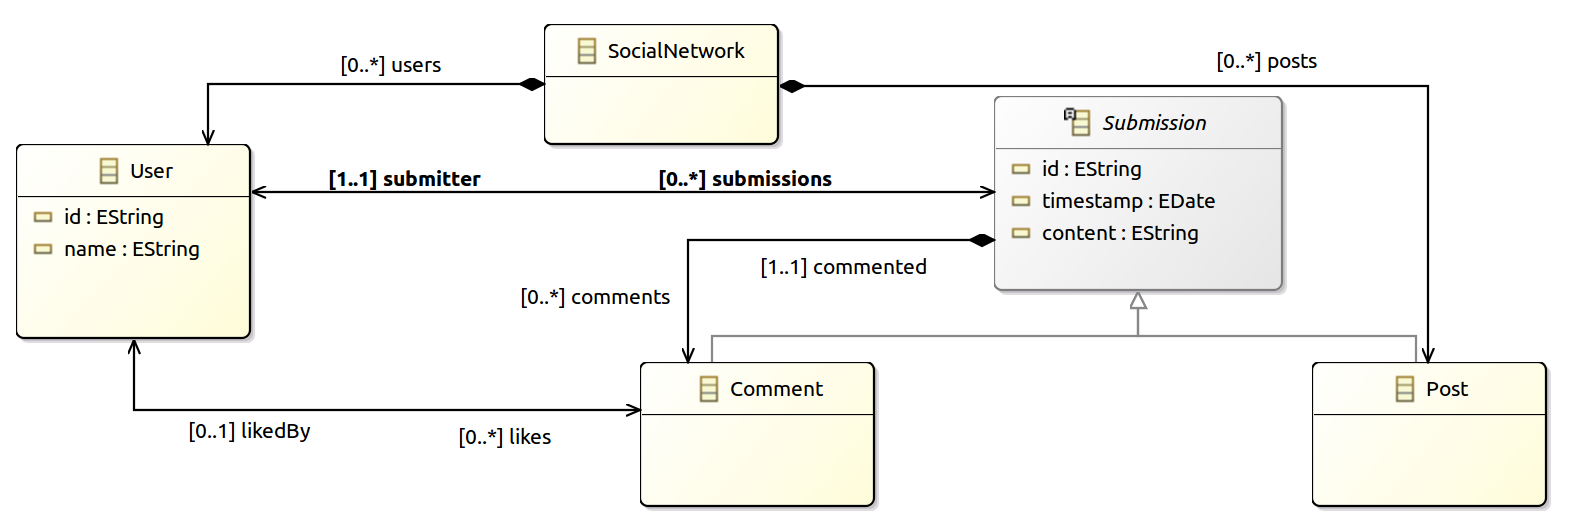
\includegraphics[scale=0.23]{figures/ttc18uml_large.png}
    \caption{The metamodel of a social network (TTC 2018)}
    \label{fig:ttc_mm}
\end{figure}   


\section{Motivating Example}
\label{sec:example}
\begin{multicols}{2}


Social network vendors often provide specific development platforms, used by developers to
build apps that extend the functionality of the social network. Some networks are associated
with marketplaces where developers can publish such apps, and end-users can buy them. 
Development platforms typically include APIs that allow analyzing and updating the social
network graph. 

As a running example for this paper, we consider a scenario where a vendor adds a LCDP to allow
end-users (also called \emph{citizen developers} in the LCDP jargon) to implement their own apps.
Such LCDP could include a `What you see is what you get editor' for the app user-interface, and a visual workflow for
the behavioral part. In particular, the LCDPs would need to provide mechanisms, at the highest
possible level of abstraction, to express queries and updates on the social graph.

In Figure~\ref{fig:ttc_mm} we show the simple metamodel for the social graph that we will use in
the paper. The metamodel has been originally proposed at the Transformation Tool Contest (TTC)
2018~\cite{Garcia2018:TTC}, and used to express benchmarks for model query and transformation
tools. In this metamodel, two main entities belong to a !SocialNetwork!. First, the !Post!s and
the !Comment!s that represent the !Submission!s, and second, the !User!s. Each !Comment! is
written by a !User!, and is necessarily attached to a !Submission! (either a !Post! or another
!Comment!). Besides commenting, the !User!s can also like !Submission!s. 

As an example, in this paper we focus on one particular query, also defined in TTC2018: the
extraction of the three most debated posts in the social network. To measure how debated is the
post, we associate it with a numeric score. The LCDP will have to provide simple and efficient
means to define and compute this score. We suppose the vendor to include a declarative query
language for expressing such computation on the social graph, and storing scores as a derived
properties of the graph (i.e. new properties of the social graph that are computed on demand
from other information in the graph). 

\end{multicols}




\section{Related Works}
\label{sec:related}

\begin{multicols}{2}
There exist attempts of using distributed strategies for running model management
operations. They can be decomposed into three main categories: data-parallelism approach,
where the full set of data is split among different processors which applies the same
computation on it; task-parallelism where each processor runs a independent computations 
that not necessary the same; and asynchronism where all data, and tasks are shared between 
processors.

\paragraph{Data-parallelism}
This computation strategy has been used by Benelallam et al.~\cite{BenelallamGTC2015:SLE}
for distributing model among computational cores to reduce cores to reduce computation time
in the ATL model transformation engine. The MapReduce version of ATL makes independent
transformations of sub-parts of the model by using a local “match-apply” function. They
highlight the good impact of their strategy for data partitioning. Instead of randomly
distributing the same number of elements among the processors, they use a strategy based
on the connectivity of models. at resolving dependencies between map outputs. Graph-based
approaches have been proposed. With this approach, the data is structured as a set of
vertices, connected by edges. For instance~\cite{Krause2014:FASE} uses Pregel, a framework
based on this approach, for computing models with a distributed strategy.

\paragraph{Task-parallelism}
In~\cite{MadaniKP2019:JOT}, Madani et al. use multi-threading for “select-based” operations
in EOL, the OCL-like language of the Epsilon framework, for querying models. In
\cite{TisiPC2013:MODELS}, Tisi et al. present a prototype of an automatic parallelization
for the ATL transformation engine, based on task-parallelism. To do so, they just use a
different thread for each transformation rule application, and each match, without taking
into account concurrency concerns (e.g., race conditions).

\paragraph{Asyncrhonism}
LinTra~\cite{BurguenoTWV2015:STAF} is a Linda-based platform for model management and has
several types of implementation. First, on a shared-memory architecture (i.e., a same shared
memory between processors, typically multi-threading solutions), LinTra proposes parallel 
transformations. Nonetheless, shared-memory architecture are fine for not too big models. 
Indeed, since the memory is not distributed, a too big model could lead to a out-of-memory 
errors. This phenomenon happens more concretely in an out-place transformation since two
models are involved during the operation. The first prototype of distributed out-place
transformations in LinTra, is presented in~\cite{BurguenoWV2016:INFSOF}.

\end{multicols}

% \section{Multi-Strategy Model Management}
% \label{sec:multistrategy}
% \begin{multicols}{2}

\end{multicols}

\section{Evaluation}
\label{sec:evaluation}
\begin{multicols}{2}
This Section gives an overview of the different strategies we use to implement the query to solve
the problem presented in Section~\ref{sec:example}. All the technical details can be found in
\cite{PhilippeCTS2020:MODELS}. First, the naive implementation is based on its OCL specification.
OCL is a standard for expressing queries, and constraints, on elements of models. It is decomposed
on several parts: first, all belonging comments of a post are recursively obtained, then all their
like is count. From these two information, the score of a post is calculated. This function has a
direct, but inefficient, counterpart. The second implementation, designed on top of Pregel, is based
on graph theory. Here, each element of the model is considered as a single element. The third
implementation works on the MapReduce paradigm: every element of the model, without considering its
type, is associated to a score. To finally obtain a score for a port, these intermediate scores a
merged into a single value. Finally, we implemented two additional approaches by mixing the one 
presented above. Some parts of the naive implementation can be optimized using the Pregel strategy.
Similarly, the MapReduce implementation can be partially replaced by an execution based on the 
graph theory of the Pregel paradigm. We experiment our five parallel implementation of the TTC18 query
(Section~\ref{sec:example}). The experiments have been conducted on a shared memory machine with a 
Intel Core i7-8650U having 8 cores at 1.90GHz and a memory of 32GB. The machine was running Ubuntu
16.04 LTS. We use Java 8, Scala 2.12 with Spark 3.1.0. Each speed-up on Table~\ref{tab:results} is
the mean of a series of 30 measures.
\end{multicols}

\begin{table}[ht]
    \centering
    \resizebox{\textwidth}{!}{
    \begin{tabular}{|c|l|l|l|l|l|c|c|c|c|c|}
        \hline
        & \multicolumn{4}{c|}{Dataset} & \multicolumn{6}{c|}{Speed-up (compared to Naive (Sequential) solution)} \\
        \hline
        & \#users & \#posts & \#comments & \#likes & Naive (Sequential) & Naive (Parallel) & Pregel & MapReduce & OCL + Pregel & MapReduce + Pregel \\
        \hline
        1 & 80 & 554 & 640 & 6 & \textbf{1x} & {\color{red} 0.40x} & {\color{dkgreen} 10.30x} & {\color{dkgreen} 5.82x} & {\color{dkgreen} 9.40x} & {\color{dkgreen} 4.63x} \\
        \hline
        2 & 889 & 1064 & 118 & 24 & \textbf{1x} & {\color{red} 0.39x} & {\color{red} 0.36x} & {\color{red} 0.46x} & {\color{red} 0.44x} & {\color{red} 0.46x} \\
        \hline
        3 & 1845 & 2315 & 190 & 66 & \textbf{1x} & {\color{red} 0.51x} & {\color{red} 0.68x} & {\color{red} 0.85x} & {\color{red} 0.66x} & {\color{red} 0.71x} \\
        \hline
        4 & 2270 & 5056 & 204 & 129 & \textbf{1x} & {\color{red} 0.27x} & {\color{red} 0.35x} & {\color{dkgreen} 2.34x} & {\color{red} 0.15x} & {\color{dkgreen} 2.96x} \\
        \hline
        5 & 5518 & 9220 & 394 & 572 & \textbf{1x} & {\color{dkgreen} 4.25x} & {\color{dkgreen} 5.21x} & {\color{dkgreen} 4.17x} & {\color{dkgreen} 4.68x} & {\color{dkgreen} 4.03x} \\
        \hline
        6 & 10929 & 18872 & 595 & 1598 & \textbf{1x} & {\color{dkgreen} 4.68x} & {\color{dkgreen} 2.83x} & {\color{dkgreen} 2.39x} & {\color{dkgreen} 1.97x} & {\color{dkgreen} 3.91x} \\
        \hline
        7 & 18083 & 39212 & 781 & 4770 & \textbf{1x} & {\color{dkgreen} 4.07x} & {\color{dkgreen} 4.12x} & {\color{dkgreen} 4.58x} & {\color{dkgreen} 5.17x} & {\color{dkgreen} 3.27x} \\
        \hline
        8 & 37228 & 76735 & 1158 & 13374 & \textbf{1x} & {\color{dkgreen} 7.28x} & {\color{dkgreen} 9.52x} & {\color{dkgreen} 7.61x} & {\color{dkgreen} 9.66x} & {\color{dkgreen} 9.22x} \\
        \hline
    \end{tabular}}
    \caption{Speed-up of 5 implementations based on different strategies for the TTC18 query}
    \label{tab:results}
\end{table}

\section{Conclusion}
\label{sec:conclusion}
% \begin{multicols}{2}
From our experiment, we observe two main points. First, using a distributed strategy generally 
look too expensive for too small data set (4 first datasets). The second observation is, 
the input data and its topology has an impact on the performances. For instance, the !Pregel!
strategy looks to have a good impact on performances for the 8th dataset, where it has a bad 
impact for the 6th dataset. The fact that the experiments have been conducted on a single machine 
can be discussed. Since Spark, the used platform is designed for Cloud architectures, we have
to conduct similar experiments on a such environment.
% \end{multicols}


\bibliography{bibliography}

\end{document}